\begin{pastexam}[label={px:ntu-112-ee-ds-11}]{臺大電機所 112 學年度 第 11 題}
（複選；每題 15 分，題內每個選項單獨計分，答對得 3 分，答錯倒扣 3 分，倒扣至複選題總分 0 分為止；未作答得 0 分，不倒扣）

There are various types of \textit{heap} data structure. Which of the following(s) is (are) a legal \textit{heap} with respect to the typename shown beside the figure?
\begin{enumerate}[label=(\Alph*)]
\item \textit{Min-Max Heap}
\item \textit{Deap}

\hspace*{2em}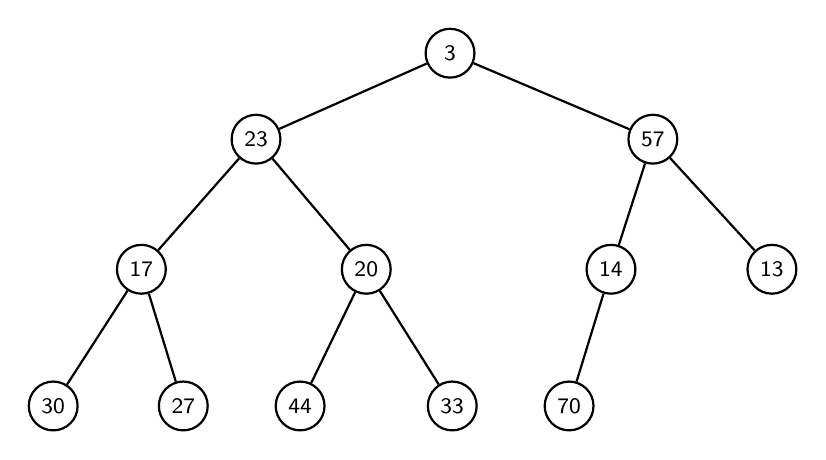
\begin{tikzpicture}[x=0.028cm,y=-0.028cm,v/.style={circle,draw,inner sep=0pt,minimum size=6.2mm,font=\small},v/.append style={font=\sffamily\footnotesize,thick}]
\node[v] (n1) at (525,713) {3};
\node[v] (n2) at (437,752) {23};
\node[v] (n3) at (617,752) {57};
\node[v] (n4) at (385,811) {17};
\node[v] (n5) at (487,811) {20};
\node[v] (n6) at (598,811) {14};
\node[v] (n7) at (671,811) {13};
\node[v] (n8) at (345,873) {30};
\node[v] (n9) at (404,873) {27};
\node[v] (n10) at (457,873) {44};
\node[v] (n11) at (526,873) {33};
\node[v] (n12) at (579,873) {70};
\draw[thick] (n1) -- (n2);
\draw[thick] (n1) -- (n3);
\draw[thick] (n2) -- (n4);
\draw[thick] (n2) -- (n5);
\draw[thick] (n3) -- (n6);
\draw[thick] (n3) -- (n7);
\draw[thick] (n4) -- (n8);
\draw[thick] (n4) -- (n9);
\draw[thick] (n5) -- (n10);
\draw[thick] (n5) -- (n11);
\draw[thick] (n6) -- (n12);
\end{tikzpicture}

\item \textit{Leftist Heap}

\hspace*{2em}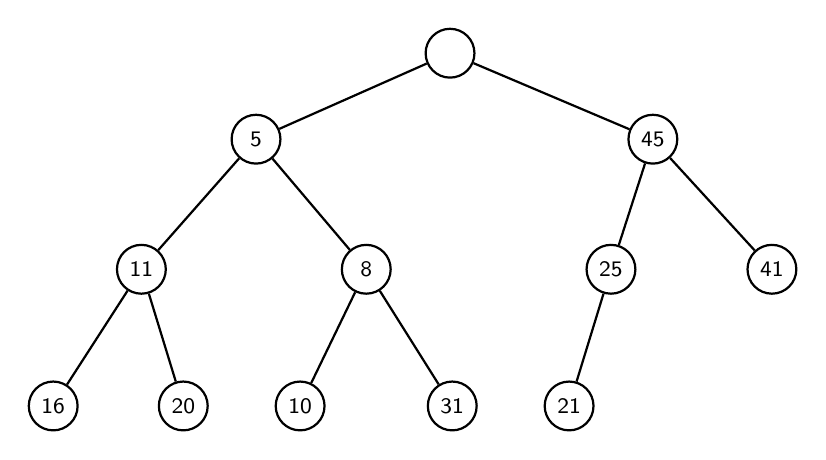
\begin{tikzpicture}[x=0.028cm,y=-0.028cm,v/.style={circle,draw,inner sep=0pt,minimum size=6.2mm,font=\small},v/.append style={font=\sffamily\footnotesize,thick}]
\node[v] (n1) at (525,713) {};
\node[v] (n2) at (437,752) {5};
\node[v] (n3) at (617,752) {45};
\node[v] (n4) at (385,811) {11};
\node[v] (n5) at (487,811) {8};
\node[v] (n6) at (598,811) {25};
\node[v] (n7) at (671,811) {41};
\node[v] (n8) at (345,873) {16};
\node[v] (n9) at (404,873) {20};
\node[v] (n10) at (457,873) {10};
\node[v] (n11) at (526,873) {31};
\node[v] (n12) at (579,873) {21};
\draw[thick] (n1) -- (n2);
\draw[thick] (n1) -- (n3);
\draw[thick] (n2) -- (n4);
\draw[thick] (n2) -- (n5);
\draw[thick] (n3) -- (n6);
\draw[thick] (n3) -- (n7);
\draw[thick] (n4) -- (n8);
\draw[thick] (n4) -- (n9);
\draw[thick] (n5) -- (n10);
\draw[thick] (n5) -- (n11);
\draw[thick] (n6) -- (n12);
\end{tikzpicture}

\item \textit{Binomial Heap}

\hspace*{2em}\begin{tikzpicture}[x=0.028cm,y=-0.028cm,v/.style={circle,draw,inner sep=0pt,minimum size=6.2mm,font=\small},v/.append style={font=\sffamily\footnotesize,thick}]
\node[v] (n3) at (529,1222) {3};
\node[v] (n5) at (440,1260) {5};
\node[v] (n11) at (387,1320) {11};
\node[v] (n16) at (348,1381) {16};
\draw[thick] (n3) -- (n5);
\draw[thick] (n5) -- (n11);
\draw[thick] (n11) -- (n16);
\end{tikzpicture}

\item \textit{Fibonacci Heap}

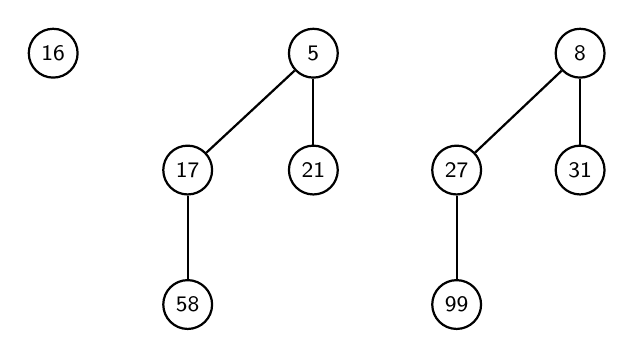
\begin{tikzpicture}[x=0.028cm,y=-0.028cm,v/.style={circle,draw,inner sep=0pt,minimum size=6.2mm,font=\small},v/.append style={font=\sffamily\footnotesize,thick}]
\node[v] (n16) at (330,360) {16};
\node[v] (n5) at (448,360) {5};
\node[v] (n8) at (569,360) {8};
\node[v] (n17) at (391,413) {17};
\node[v] (n21) at (448,413) {21};
\node[v] (n27) at (513,413) {27};
\node[v] (n31) at (569,413) {31};
\node[v] (n58) at (391,474) {58};
\node[v] (n99) at (513,474) {99};
\draw[thick] (n5) -- (n17);
\draw[thick] (n5) -- (n21);
\draw[thick] (n17) -- (n58);
\draw[thick] (n8) -- (n27);
\draw[thick] (n8) -- (n31);
\draw[thick] (n27) -- (n99);
\end{tikzpicture}

\vspace{8mm}
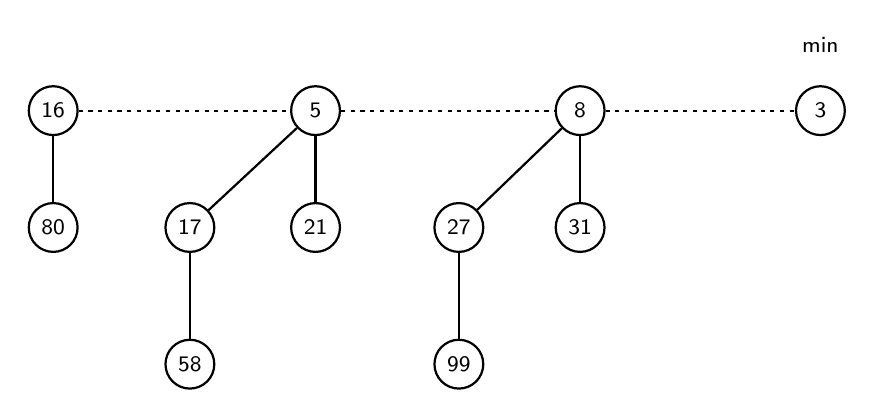
\begin{tikzpicture}[x=0.028cm,y=-0.028cm,v/.style={circle,draw,inner sep=0pt,minimum size=6.2mm,font=\small},v/.append style={font=\sffamily\footnotesize,thick}]
\node[v] (n16) at (329,595) {16};
\node[v] (n5) at (448,595) {5};
\node[v] (n8) at (568,595) {8};
\node[v] (n3) at (677,595) {3};
\node[v] (n80) at (329,648) {80};
\node[v] (n17) at (391,648) {17};
\node[v] (n21) at (448,648) {21};
\node[v] (n27) at (513,648) {27};
\node[v] (n31) at (568,648) {31};
\node[v] (n58) at (391,710) {58};
\node[v] (n99) at (513,710) {99};
\draw[thick] (n16) -- (n80);
\draw[thick] (n5) -- (n17);
\draw[thick] (n5) -- (n21);
\draw[thick] (n17) -- (n58);
\draw[thick] (n8) -- (n27);
\draw[thick] (n8) -- (n31);
\draw[thick] (n27) -- (n99);
\draw[thick,dash pattern=on 1.5pt off 2pt] (n16) -- (n5) -- (n8) -- (n3);
\node[font=\sffamily\footnotesize] at (677,565) {min};
\end{tikzpicture}
\end{enumerate}
\end{pastexam}

\begin{pastsoln}
答案是 (B)(C)(E)（採用下面說明的讀法）。

\textbf{先說明題目的排版問題。} 原卷 (A)、(B) 兩個標籤連在一起，下面才是第一張圖；(E) 下面則有兩張圖。 照
「標籤下面的圖屬於它」去讀，(A) 沒有圖可以判斷。 看圖的樣子：第二張圖的根是空的，正是 deap 的畫法；最後
一張圖有虛線串起的根串列和 min 指標，正是費氏堆積的畫法。 所以本書採用的讀法是：五張圖依序對應 (A)--(E)，
每張圖都排在下一個標籤後面：
\begin{center}
\small
\begin{tabular}{lll}
\toprule
選項 & 圖 & 判斷 \\
\midrule
(A) Min-Max Heap & 根為 $3$ 的 $12$ 個節點的樹 & 不合法 \\
(B) Deap & 根是空的那棵樹 & 合法 \\
(C) Leftist Heap & $3 - 5 - 11 - 16$ 一路往左的鏈 & 合法 \\
(D) Binomial Heap & 沒有根串列的三棵樹 $16$；$5$；$8$ & 不合法 \\
(E) Fibonacci Heap & 有 min 指標的四棵樹 & 合法 \\
\bottomrule
\end{tabular}
\end{center}
若照字面讀（第一張圖給 (B)、第二張給 (C)、鏈給 (D)、兩張都給 (E)），只有 (E) 合法：根有元素的樹不是 deap、
根是空的樹不是左傾樹、一條鏈不是二項樹。 下面逐項說明本書採用的讀法。

\textbf{(A) 最小最大堆積：錯。} 定義見資結書第~8.5~節：深度 $0, 2, \ldots$ 是最小層，深度 $1, 3, \ldots$ 是最大層；
最小層的節點不大於所有子孫，最大層的節點不小於所有子孫。 圖中深度 $1$（最大層）的 $23$，子孫有
$17, 20, 30, 27, 44, 33$，其中 $30, 27, 44, 33$ 都比 $23$ 大，違反最大層的條件；另一個最大層節點 $57$ 也比它的
孫子 $70$ 小。 所以不是最小最大堆積。

\textbf{(B) deap：對。} 照資結書第~8.5.2~節的陣列編號，根 $A[1]$ 空著，$\mathit{last} = 12$，
\[
A[2..12] = \langle 5, 45, 11, 8, 25, 41, 16, 20, 10, 31, 21\rangle .
\]
\begin{itemize}
\item 左子樹（最小堆積）：$5 \le 11, 8$；$11 \le 16, 20$；$8 \le 10, 31$。 成立。
\item 右子樹（最大堆積）：$45 \ge 25, 41$；$25 \ge 21$。 成立。
\item 對應點 $j = i + 2^{\lfloor \lg i \rfloor - 1}$，超出 $\mathit{last}$ 就改用 $\lfloor j/2 \rfloor$：
$A[2] = 5 \le A[3] = 45$；$A[4] = 11 \le A[6] = 25$；$A[5] = 8 \le A[7] = 41$；$A[8] = 16 \le A[12] = 21$；
$A[9] = 20$ 的對應點 $13$ 超出，改用 $6$，$20 \le 25$；$A[10] = 10$、$A[11] = 31$ 的對應點 $14, 15$ 超出，
改用 $7$，$10 \le 41$、$31 \le 41$。 全部成立。
\end{itemize}
所以是合法的 deap。

\textbf{(C) 左傾堆積：對。} 鏈上每個節點都是上一個的\textbf{左}子節點，鍵 $3 < 5 < 11 < 16$，滿足最小堆積。
每個節點的右子樹是空的，$s(\text{右}) = 0 \le s(\text{左})$，左傾條件成立（資結書第~8.5~節左傾樹的定義）。
一路往左的鏈正是最「左傾」的形狀，合法。

\textbf{(D) 二項堆積：錯。} 三棵樹：$16$ 是 $B_0$；$5[17[58],\,21]$ 和 $8[27[99],\,31]$ 都是 $B_2$（根有兩棵子樹，
分別是 $B_1$ 和 $B_0$），各自也滿足最小堆積。 但二項堆積規定\textbf{每個階數最多一棵樹}（資結書第~8.5~節），
這裡有兩棵 $B_2$，所以不是。 （元素個數 $9 = 1001_2$，合法的二項堆積應該是一棵 $B_3$ 加一棵 $B_0$。）
注意：有些課本把二項堆積寫成延遲合併的版本，平時允許同階的樹並存，等取出最小值時才合併；照那種定義這張圖
可以算合法。 本書照一般（CLRS）的定義判錯。

\textbf{(E) 費氏堆積：對。} 根串列是 $16, 5, 8, 3$，每棵樹都滿足最小堆積（$16 < 80$；$5 < 17 < 58$、$5 < 21$；
$8 < 27 < 99$、$8 < 31$），min 指標指向最小的根 $3$。 費氏堆積不要求樹的形狀，同階的樹可以並存，只要堆積
順序對、min 指標對就合法（資結書第~8.6~節）。
\end{pastsoln}
